\chapter{Evaluation}\label{chapter:evaluation}
In this chapter, we evaluate the performance of our code generating regular expression engine prototype in comparison to other popular C++ regular expressions engines. All the benchmarks were run on a server with a twenty core Intel(R) Core(TM) i9-7900X @ 3.30GHz processor, 128 GiB RAM running Ubuntu 21.10.

\newcounter{magicrownumbers1}
\newcounter{magicrownumbers2}
\newcommand\rownumberone{\stepcounter{magicrownumbers1}\arabic{magicrownumbers1}}
\newcommand\rownumbertwo{\stepcounter{magicrownumbers2}\arabic{magicrownumbers2}}

\section{DFA Compilation Time Evaluation}
In this section, We evaluate the compilation time for the two backends \textbf{\{LLVM, CPP\}} and the two Unicode encoding mechanisms \textbf{\{UTF-8, UTF-32\}}.

\subsection{Common Patterns Benchmark}
RegExLib \cite{regexlib} is a popular Regular Expressions repository on the Web, with expressions for matching URIs, HTML code, C style strings, Java code, SQL queries, spam, and so on. We extracted the top ten non-duplicate patterns from RegExLib to use in this benchmark. In this benchmark, we test for each backend and encoding mechanism how long does it take to compile the input pattern to a DFA and then generate the pattern matching code. 

The results of this benchmark is shown in Figure \ref{fig:eval_common}. These results show what we expected that the LLVM backend compilation is $\mathbf{9x}$ faster than C++ code with both encodings. This is due to the fact that when generating LLVM code everything is done in memory and no CPU time is wasted while for C++ we had to write the code to the disk, wait for the \texttt{clang} compiler to execute then read the generated IR again. It also shows that for this benchmark, UTF-32 encoding is slightly faster at $\mathbf{1.2x}$ that of UTF-8 encoding since it generates smaller overall automatons.

{\renewcommand{\arraystretch}{1.5}% for the vertical padding
\begin{table}[H]
\centering
\small
\begin{tabularx}{\textwidth}{|l|X|}
\hline
& Pattern       \\
\hline
\rownumbertwo & \texttt{\textbf{{[}a-zA-Z0-9 {]}*}}\\ \hline
\rownumbertwo & \texttt{\textbf{{[}2-9{]}{[}0-9{]}\{2\}-{[}0-9{]}\{3\}-{[}0-9{]}\{4\}}}\\ \hline
\rownumbertwo & \texttt{\textbf{{[}a-zA-Z0-9.\_\%-{]}+@{[}a-zA-Z0-9.-{]}+.{[}a-zA-Z{]}\{2,6\}}}\\ \hline
\rownumbertwo & \texttt{\textbf{{[}0-9{]}*.?{[}0-9{]}*}}\\ \hline
\rownumbertwo & \texttt{\textbf{({[}0-1{]}{[}0-9{]}|{[}2{]}{[}0-3{]}):({[}0-5{]}{[}0-9{]})}}\\ \hline
\rownumbertwo & \texttt{\textbf{({[}0-9{]}\{3\})?|({[}0-9{]}\{3\})({[}-./{]}?)({[}0-9{]}\{3\})({[}0-9-./{]}?)({[}0-9{]}\{4\})}}\\ \hline
\rownumbertwo & \texttt{\textbf{{[}-+{]}?{[}0-9{]}+{[}.{]}?{[}0-9{]}*({[}eE{]}{[}-+{]}?{[}0-9{]}+)?}}\\ \hline
\rownumbertwo & \texttt{\textbf{({[}0-9{]}\{1,2\}|1{[}0-9{]}{[}0-9{]}|2{[}0-4{]}{[}0-9{]}|25{[}0-5{]})({[}0-9{]}\{1,2\}|1{[}0-9{]}{[}0-9{]}|2{[}0-4{]}{[}0-9{]}|25{[}0-5{]})({[}0-9{]}\{1,2\}|1{[}0-9{]}{[}0-9{]}|2{[}0-4{]}{[}0-9{]}|25{[}0-5{]})({[}0-9{]}\{1,2\}|1{[}0-9{]}{[}0-9{]}|2{[}0-4{]}{[}0-9{]}|25{[}0-5{]}) }}\\ \hline
\rownumbertwo & \texttt{\textbf{{[}a-zA-Z0-9@*\#{]}\{8,15\}}}\\ \hline
\rownumbertwo & \texttt{\textbf{{[}0-9{]}\{1,3\}(,{[}0-9{]}\{3\})*|({[}0-9{]}+)(.{[}0-9{]}\{2\})?}}\\
\hline

\end{tabularx}
\caption{Patterns in the Common Patterns Benchmark.}\label{tab:cmpbench}
\end{table}}


\begin{figure}[H]
\hspace*{-45pt}

\centering
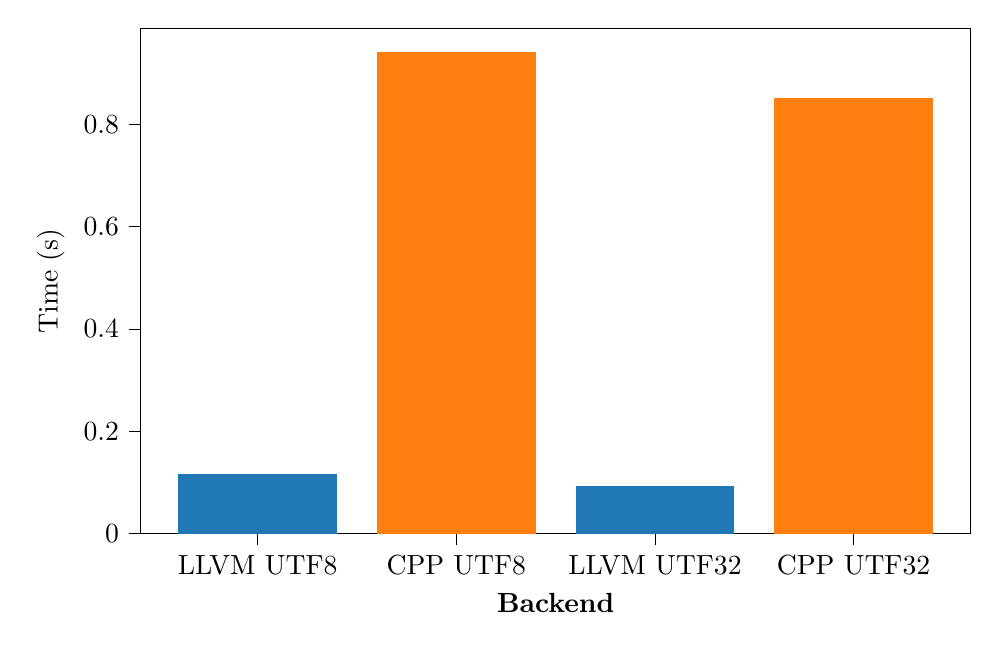
\begin{tikzpicture}
\definecolor{darkgray176}{RGB}{176,176,176}
\definecolor{darkorange25512714}{RGB}{255,127,14}
\definecolor{steelblue31119180}{RGB}{31,119,180}
\begin{axis}[
% scale only axis,
width={\textwidth},
% height=\axisdefaultheight,
height=8cm,
tick align=outside,
tick pos=left,
x grid style={darkgray176},
xlabel={\textbf{Backend}},
xmin=-0.59, xmax=3.59,
xtick style={color=black},
xtick={0,1,2,3},
xticklabels={LLVM UTF8,CPP UTF8,LLVM UTF32,CPP UTF32},
y grid style={darkgray176},
ylabel={Time (s)},
ymin=0, ymax=0.988243550527841,
ytick style={color=black}
]
\draw[draw=none,fill=steelblue31119180] (axis cs:-0.4,0) rectangle (axis cs:0.4,0.11753389959534);
\draw[draw=none,fill=darkorange25512714] (axis cs:0.6,0) rectangle (axis cs:1.4,0.941184333836039);
\draw[draw=none,fill=steelblue31119180] (axis cs:1.6,0) rectangle (axis cs:2.4,0.0936958231031895);
\draw[draw=none,fill=darkorange25512714] (axis cs:2.6,0) rectangle (axis cs:3.4,0.852185526241859);
\end{axis}

\end{tikzpicture}

\caption{Compilation time performance for the Common Patterns Benchmark. Statistic is mean ($\mu$). Time in seconds (s).}
\label{fig:eval_common}
\end{figure}



\subsection{GitHub SQL Benchmark}
The results from the previous benchmark were promising and aligned with our expectations. To further test our assumptions, we created another benchmark by scraping $524$ regular expressions from open-source SQL projects on GitHub. These projects were SQL projects and patterns are SQL-flavored regular expressions. $77$ of these patterns contain Unicode characters which would showcase the performance of the engine on Unicode. Table \ref{tab:samplesql} shows a sample of these patterns.

{\renewcommand{\arraystretch}{1.5}% for the vertical padding
\begin{table}[H]
\centering
\small
\begin{tabularx}{\textwidth}{|l|X|}
\hline
& Pattern       \\
\hline
\rownumberone & \texttt{\textbf{{[}{[}:ALNUM:{]}.\_\%+-{]}+@{[}{[}:ALNUM:{]}.-{]}+.{[}{[}:ALPHA:{]}{]}+}} \\
\hline
\rownumberone & \texttt{\textbf{\${[}0-9{]}+(.{[}0-9{]}{[}0-9{]})?}}                                      \\
\hline
\rownumberone &\texttt{\textbf{\%AK Email Signup\%}}                                                     \\
\hline
\rownumberone &\texttt{\textbf{\%Assistant\%(I)*}}                                                       \\
\hline
\rownumberone &\texttt{\textbf{{[}A-Z{]}{[}0-9{]}\{3\}-{[}0{]}{[}A-Z{]}\{2\}}}                          \\
\hline
\rownumberone & \texttt{\textbf{\%(汉服|国创|国漫|国潮|姜子牙|哪吒|东方美|中国风)\%}}     \\            
\hline
\end{tabularx}
\caption{Sample of the patterns in the Github SQL Benchmark.}\label{tab:samplesql}
\end{table}}

Figure \ref{fig:eval_sql} the results of the benchmark. The results again show the compilation performance difference for LLVM and CPP backends. LLVM backend compilation is again $\mathbf{~9x}$ faster than C++ code with both encodings. An interesting result here we see the performance for UTF-8 is $\mathbf{2x}$ faster than UTF-32 for LLVM and $\mathbf{1.6}x$ faster for CPP Backend. This is in contrary to the results from the first benchmark. The reason for this change is the Unicode patterns, While the UTF32 backend generates smaller automatons than UTF-8 It has to read and verify the whole Unicode codepoint when compiling that takes extra time and is slower than UTF8 that treats everything as a byte. To confirm that this is the reason, we removed the Unicode patterns from the list and the result was the UTF-32 encoding was $\mathbf{1.36x}$ faster than UTF-8 for LLVM and $\mathbf{1.22x}$ for C++ Backend.

\begin{figure}[H]
\centering
\hspace*{-45pt}
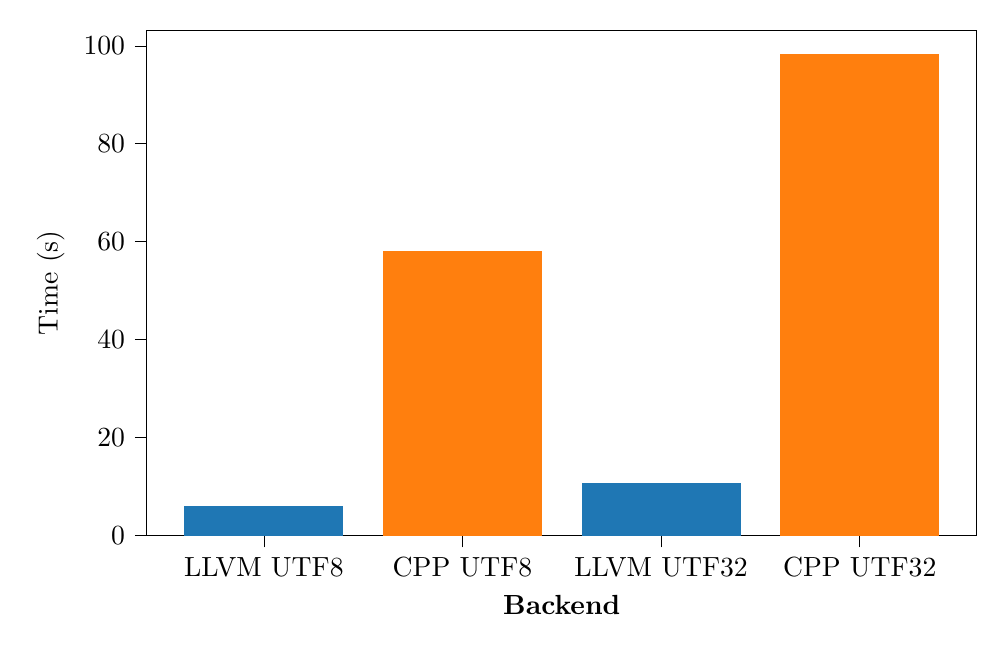
\begin{tikzpicture}

\definecolor{darkgray176}{RGB}{176,176,176}
\definecolor{darkorange25512714}{RGB}{255,127,14}
\definecolor{steelblue31119180}{RGB}{31,119,180}

\begin{axis}[
% scale only axis,
width={\textwidth},
height=8cm,
tick align=outside,
tick pos=left,
x grid style={darkgray176},
xlabel={\textbf{Backend}},
xmin=-0.59, xmax=3.59,
xtick style={color=black},
xtick={0,1,2,3},
xticklabels={LLVM UTF8,CPP UTF8,LLVM UTF32,CPP UTF32},
y grid style={darkgray176},
ylabel={Time (s)},
ymin=0, ymax=103.19825138282,
ytick style={color=black}
]
\draw[draw=none,fill=steelblue31119180] (axis cs:-0.4,0) rectangle (axis cs:0.4,5.96466026082635);
\draw[draw=none,fill=darkorange25512714] (axis cs:0.6,0) rectangle (axis cs:1.4,58.0985493951788);
\draw[draw=none,fill=steelblue31119180] (axis cs:1.6,0) rectangle (axis cs:2.4,10.7183447480202);
\draw[draw=none,fill=darkorange25512714] (axis cs:2.6,0) rectangle (axis cs:3.4,98.2840489360193);
\end{axis}
\end{tikzpicture}
\caption{Compilation time performance for the Github SQL Benchmark.}
\label{fig:eval_sql}
\end{figure}

In conclusion, these two benchmarks confirmed our assumptions regarding the compilation time that LLVM backend code-generation is much faster than C++. It also showed while in the average use case where patterns are mostly ASCII only the UTF-32 encoding compiles faster, UTF-8 is faster to compile when dealing with lots of Unicode code-points in the pattern.

\section{Matching Performance Evaluation}

In this section, We evaluate the performance of our prototype engine (with its two backends and encoding mechanisms) against other popular C++ regular expressions engines \textbf{\{RE2, PCRE2, Boost\}}.

\subsection{Engines}

RE2 \cite{re2} is a C++ software library for regular expressions developed and used by Google. It uses a finite-state machine based matching that guarantees that run-time increases linearly (not exponentially) with the size of the input.

PCRE2 \cite{pcre2} is a regular expressions matching library for the C programming language. PCRE's syntax is much more powerful and flexible that of RE2 and many other regular-expression libraries. It uses backtracking as its matching algorithm. In this benchmark, we use PCRE2 with JIT support. We discuss PCRE2 JIT Support in Chapter \ref{chapter:related_work}.

Boost Regex \cite{Boost} is a C++ Regular Expressions Library. It is part of the standard library since C++11. Similar to PCRE2, It uses backtracking algorithm for matching. In this benchmark, we explicitly use Boost version of the library not the one shipped with the \texttt{\textbf{stdlib}} due to a bug in the implementation with long text \footnote{\url{https://gcc.gnu.org/bugzilla/show\_bug.cgi?id=86164}}.

\subsection{TPC-H Benchmark}
TPC-H \cite{tpch} is a benchmark for decision support. It is composed of a set of business-oriented ad-hoc queries and concurrent data modifications.
In this benchmark, we test the sub-string matching of the different engines. In particular we use Query 13 that try to find all rows where the field \texttt{\textbf{o\_comment}} matches the pattern \texttt{\textbf{\%special\%packages\%}} in the \texttt{\textbf{orders}} table. The table has around $1.5$ million rows.

\begin{figure}[H]
    \centering
    \hspace*{-45pt}
    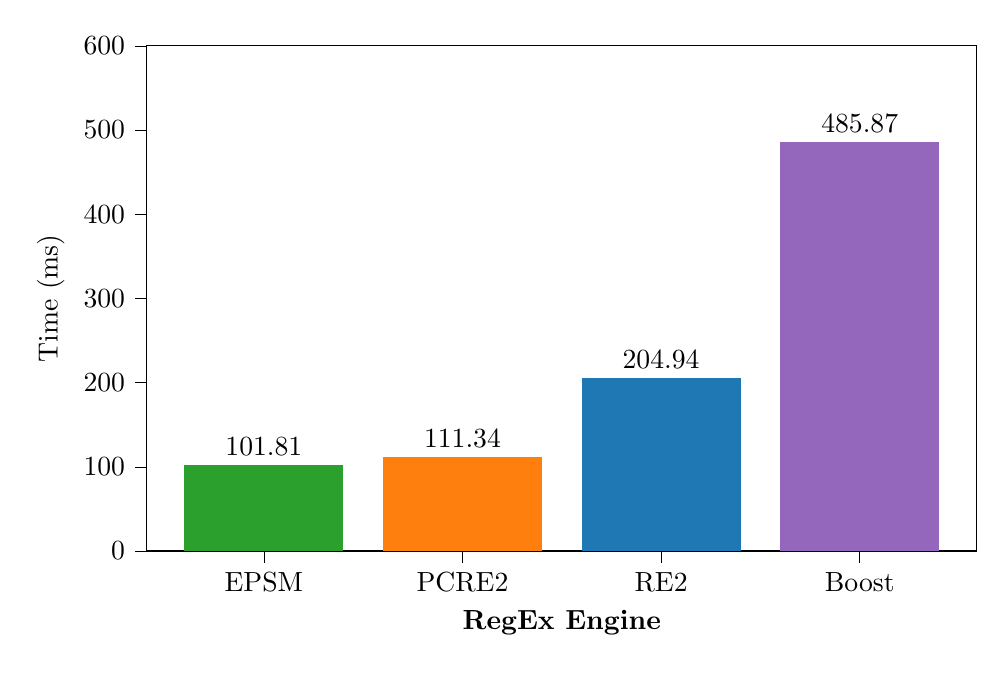
\begin{tikzpicture}
    \definecolor{crimson2143940}{RGB}{214,39,40}
    \definecolor{darkgray176}{RGB}{176,176,176}
    \definecolor{darkorange25512714}{RGB}{255,127,14}
    \definecolor{forestgreen4416044}{RGB}{44,160,44}
    \definecolor{lightgray204}{RGB}{204,204,204}
    \definecolor{mediumpurple148103189}{RGB}{148,103,189}
    \definecolor{sienna1408675}{RGB}{140,86,75}
    \definecolor{steelblue31119180}{RGB}{31,119,180}

\begin{axis}[
    width=\textwidth,
    height=8cm,
    tick align=outside,
    tick pos=left,
    x grid style={darkgray176},
    xlabel={\textbf{RegEx Engine}},
    xmin=-0.59, xmax=3.59,
    xtick style={color=black},
    xtick={0,1,2,3},
    xticklabels={EPSM, PCRE2, RE2, Boost},
    y grid style={darkgray176},
    ylabel={Time (ms)},
    ymin=0, ymax=600.172420926392,
    ytick style={color=black}
    ]
        
    \draw[draw=none,fill=forestgreen4416044] (axis cs:-0.4,0) rectangle (axis cs:0.4,101.814205093043);
    \draw[draw=none,fill=darkorange25512714] (axis cs:0.6,0) rectangle (axis cs:1.4,111.341547738347);
    \draw[draw=none,fill=steelblue31119180] (axis cs:1.6,0) rectangle (axis cs:2.4,204.944238894516);
    \draw[draw=none,fill=mediumpurple148103189] (axis cs:2.6,0) rectangle (axis cs:3.4,485.878496120373);
    \draw (axis cs:0,101.814205093043) ++(0pt,0pt) node[
      scale=1,
      anchor=south,
      text=black,
      rotate=0.0
    ]{101.81};
    \draw (axis cs:1,111.341547738347) ++(0pt,0pt) node[
      scale=1,
      anchor=south,
      text=black,
      rotate=0.0
    ]{111.34};
    \draw (axis cs:2,204.944238894516) ++(0pt,0pt) node[
      scale=1,
      anchor=south,
      text=black,
      rotate=0.0
    ]{204.94};
    \draw (axis cs:3,485.878496120373) ++(0pt,0pt) node[
      scale=1,
      anchor=south,
      text=black,
      rotate=0.0
    ]{485.87};
    \end{axis}
    \end{tikzpicture}
    \caption{Matching performance on TPC-H Q13.}
    \label{fig:tpchres}
\end{figure}

Figure \ref{fig:tpchres} shows the performance of the different engines on this benchmark. The results shows our implementation with EPSM algorithm was the fastest beating the heavily RE2 optimized with a speedup of $1.27x$ and PCRE2 with a factor of $1.1x$. All the engines (Ours, RE2 and PCRE2) were much faster than the baseline Boost achieving $4.8x$, $2.37x$ and $4.36x$ respectively.

\subsection{Regex-Redux Benchmark}
Regex-Redux \cite{regexredux} is a benchmark that consists of nine simple patterns that represent DNA 8-mers and their reverse and a dataset that consists $90k$ rows of DNA Sequences.


{\renewcommand{\arraystretch}{1.2}% for the vertical padding
\begin{table}[H]
\centering
\begin{adjustbox}{width=1.3\textwidth,center=\textwidth}
\begin{tabular}{|l|c|c|c|c|c|c|c|}
\hline
\diagbox{Pattern}{Engine} & RE2 & PCRE2 & DFA LLVM U8 & DFA LLVM U32 & DFA CPP U8 & DFA CPP U32 & Boost \\
\hline
agggtaaa|tttaccct & 15.07 & \bfseries 13.31 & 45.30 & 44.15 & 137.92 & 93.33 & 117.58 \\\hline
[cgt]gggtaaa|tttaccc[acg] & \bfseries 15.09 & 15.75 & 45.05 & 41.45 & 138.93 & 102.58 & 142.52 \\\hline
a[act]ggtaaa|tttacc[agt]t & \bfseries 15.03 & 16.37 & 49.20 & 43.44 & 139.48 & 98.25 & 147.23 \\\hline
agg[act]taaa|ttta[agt]cct & 19.23 & \bfseries 16.34 & 56.56 & 51.94 & 137.35 & 102.31 & 118.68 \\\hline
aggg[acg]aaa|ttt[cgt]ccct & 15.02 & \bfseries 13.88 & 49.38 & 41.42 & 158.61 & 137.38 & 118.15 \\\hline
agggtaa[cgt]|[acg]ttaccct & \bfseries 15.03 & 19.87 & 55.69 & 49.81 & 148.95 & 112.38 & 144.80 \\\hline
agggta[cgt]a|t[acg]taccct & \bfseries 15.05 & 16.40 & 56.02 & 42.12 & 148.41 & 104.81 & 137.60 \\\hline
agggt[cgt]aa|tt[acg]accct & 15.27 & \bfseries 15.12 & 47.82 & 45.59 & 145.88 & 105.82 & 121.08 \\\hline
ag[act]gtaaa|tttac[agt]ct & 14.92 & \bfseries 14.43 & 52.87 & 47.04 & 152.28 & 97.14 & 119.82 \\\hline
\end{tabular}
\end{adjustbox}
\caption{Performance Evaluation results on RegexDNA Benchmark. \\Statistic is Mean ($\mu$). Time in Milliseconds (ms).}\label{tab:evalrgxdna}
\end{table}}


We use this benchmark as a baseline for performance analysis. We test the engines and how would they behave on a simple benchmark with small number of rows and the effect of JIT compilation. 

Table \ref{tab:evalrgxdna} shows the performance results for each pattern in the benchmark. RE2 and PCRE2 had the best performance. The results show that when the number of rows is small as in this benchmark and the patterns are also simple, the code generation and compilation time negatively affect the performance and Interpreted code is faster.

\subsection{Logs Benchmark}

LogHub \cite{loghub} maintains a collection of system logs, which are freely accessible for research purposes. Some of the logs are from prior studies' production data, while others are from genuine systems in our lab environment. The logs are NOT cleaned, anonymised, or altered in any manner if possible.

In this benchmark, we used the \textit{Spark Logs} dataset from Loghub which contains 33,236,604 log message from Spark jobs. Table \ref{tab:pattlogbench} shows the four patterns we applied to this dataset to evaluate the performance of the engines. It also shows what each pattern does and the number of expected matches for each pattern. It should be noted that the patterns may not be strictly correct or ideal. We simply require something to test the performance.

This benchmark represents a real-scenario for our use-case with millions of rows and patterns that aren't too complex but useful for analysis.

{\renewcommand{\arraystretch}{1.5}% for the vertical padding
\begin{table}[H]
\centering
% \begin{adjustbox}{width=1.2\textwidth,center=\textwidth}
\small
\makebox[\textwidth]{%
\begin{tabularx}{1.25\textwidth}{|X|l|l|}
\hline
Pattern & Description & Matches\\
\hline
\texttt{\textbf{({[}a-zA-Z{]}{[}a-zA-Z0-9{]}*)://({[}\textasciicircum /{]}+)(/{[}\textasciicircum  {]}*)?}} & URI (protocol://server/path) & 793,701\\ \hline

\texttt{\textbf{{[}a-zA-Z0-9\_.+-{]}+@{[}a-zA-Z0-9-{]}+{[}.{]}{[}a-zA-Z0-9-.{]}+}} & Email &  15,002\\ \hline

\texttt{\textbf{({[}0-9{]}{[}0-9{]}?)/({[}0-9{]}{[}0-9{]}?)/({[}0-9{]}{[}0-9{]}({[}0-9{]}{[}0-9{]})?)}} & Date (day/month/year) & 27,410,266\\ \hline

\texttt{\textbf{({[}a-zA-Z{]}{[}a-zA-Z0-9{]}*)://({[}\textasciicircum /{]}+)(/{[}\textasciicircum {]}*)?|{[}a-zA-Z0-9\_.+-{]}+@{[}a-zA-Z0-9-{]}+{[}.{]}{[}a-zA-Z0-9-.{]}+}} & URI or Email & 793,802\\
\hline
\end{tabularx}}
% \end{adjustbox}
\caption{Patterns Used in Log Benchmark and Number of Matches.}\label{tab:pattlogbench}
\end{table}
}

Table \ref{tab:evallogbench} shows the results of the benchmark for each pattern and engine under test. Boost was the worst performing engine by a factor of $20x-40x$ in comparison to the other engines so we exclude it from the analysis as it struggles with large data-sets and not suitable for our use-case. Figure \ref{fig:graphlogbench} shows the results with Boost Engine excluded.

{\renewcommand{\arraystretch}{1.6}% for the vertical padding
\begin{table}[H]
\centering
\begin{adjustbox}{width=1.2\textwidth,center=\textwidth}
\large
\begin{tabular}{|l|l|l|l|l|l|l|l|l|}
\hline
\diagbox{Pattern}{Engine} & RE2 & PCRE2 & DFA LLVM U8 & DFA LLVM U32 & DFA CPP U8 & DFA CPP U32 & Boost\\
\hline
URI (protocol://server/path) & 6.76 & \bfseries 2.67 & 6.31 & 9.57 & 6.71 & 9.16 & 105.27\\ \hline
Email & 6.84 & \bfseries 5.56 & 6.29 & 9.74 & 6.52 & 9.83 & 102.95\\ \hline
Date (day/month/year) & 3.21 & 2.40 & \bfseries 1.78 & 2.28 & 1.83 & 2.15 & 34.53 \\ \hline
URI or Email & 6.73 & 16.86 & \bfseries 6.15 & 10.12 & 6.15 & 9.75 & 192.92\\ \hline
\end{tabular}
\end{adjustbox}
\caption{Performance Evaluation results on Logs Benchmark. \\Statistic is Mean ($\mu$). Time in Seconds.}\label{tab:evallogbench}
\end{table}
}

For the first pattern that recognizes URIs, it matches $2.37\%$ of the rows and the best performing engine was PCRE2 and was faster by a factor of $2.36x$ than the second best engine which is our UTF-8 LLVM implementation. Still both engines were faster than the heavily optimized RE2. The results show that JIT compilation was beneficial and the compilation time was amortized over the large number of times the matching function was used. 

The second pattern recognizes Emails matches less than $0.004\%$ of the rows. Again PCRE2 was the fastest engine but by a smaller factor of $1.13x$ than the second best engine. They both once again were faster than RE2. The drop in performance for PCRE2 can be explained by the much smaller number of matches and therefore a lot of time was spent navigating the text.

The third pattern is used to recognize Date. Every log line starts with the date therefore, it matches $82.4\%$ of the lines (since a log can span multiple lines). Our Implementation was the fastest on this with a factor of $1.34x$ than the second engine PCRE2. This speedup in our engine is due to our early termination in the engine Where, we don't process the line once a match was found and report success immediately.

The fourth and last pattern is an alternation of the first and second pattern and recognizes either a URI or an email. It matches $2.38\%$ of the rows. The performance of PCRE2 suddenly dropped on this pattern and the best performing was our implementation followed by RE2. This can be attributed to the fact that PCRE2 use a backtracking algorithm which usually struggles with alternations since it has to try both paths.



\begin{figure}[H]
    \centering
    \hspace*{-45pt}
    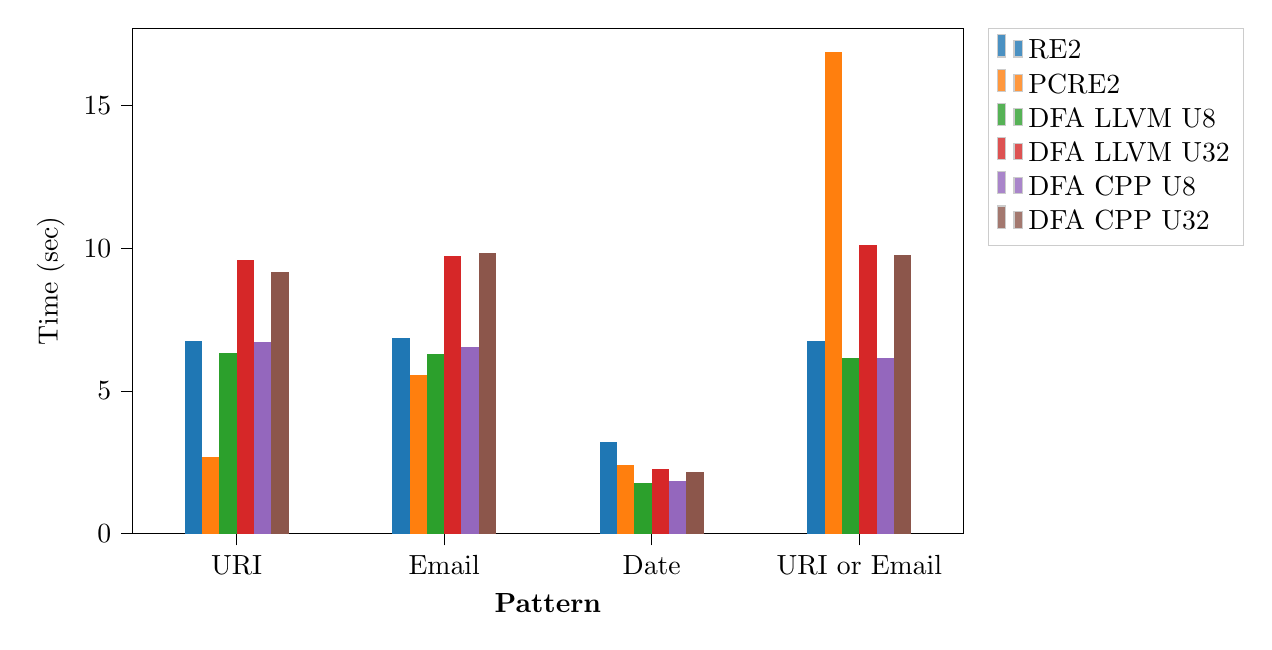
\begin{tikzpicture}
    \definecolor{crimson2143940}{RGB}{214,39,40}
    \definecolor{darkgray176}{RGB}{176,176,176}
    \definecolor{darkorange25512714}{RGB}{255,127,14}
    \definecolor{forestgreen4416044}{RGB}{44,160,44}
    \definecolor{lightgray204}{RGB}{204,204,204}
    \definecolor{mediumpurple148103189}{RGB}{148,103,189}
    \definecolor{sienna1408675}{RGB}{140,86,75}
    \definecolor{steelblue31119180}{RGB}{31,119,180}
    
    \begin{axis}[
    legend cell align={left},
    legend style={
      fill opacity=0.8,
      draw opacity=1,
      text opacity=1,
    %   at={(0.03,0.97)},
        % at={(-0.5,-0.5)},
      anchor=north west,
      legend pos= outer north east,
      draw=lightgray204,
    },
    % scale axis only,
    bar width=9pt,
    width=\textwidth,
    height=8cm,
    tick align=outside,
    tick pos=left,
    x grid style={darkgray176},
    xlabel={\textbf{Pattern}},
    xmin=-0.5, xmax=3.5,
    xtick style={color=black},
    xtick={0,1,2,3},
    xticklabel style={rotate=0},
    xticklabels={URI,Email,Date,URI or Email},
    y grid style={darkgray176},
    ymin=0, ymax=17.7023160803132,
    ytick style={color=black},
    ylabel={Time (sec)}
    ]
    \draw[draw=none,fill=steelblue31119180] (axis cs:-0.25,0) rectangle (axis cs:-0.166666666666667,6.75804211944342);
    \addlegendimage{ybar,ybar legend,draw=none,fill=steelblue31119180}
    \addlegendentry{RE2}
    
    \draw[draw=none,fill=steelblue31119180] (axis cs:0.75,0) rectangle (axis cs:0.833333333333333,6.83566853404045);
    \draw[draw=none,fill=steelblue31119180] (axis cs:1.75,0) rectangle (axis cs:1.83333333333333,3.20648544281721);
    \draw[draw=none,fill=steelblue31119180] (axis cs:2.75,0) rectangle (axis cs:2.83333333333333,6.73386627311508);
    \draw[draw=none,fill=darkorange25512714] (axis cs:-0.166666666666667,0) rectangle (axis cs:-0.0833333333333333,2.66720288681487);
    \addlegendimage{ybar,ybar legend,draw=none,fill=darkorange25512714}
    \addlegendentry{PCRE2}
    
    \draw[draw=none,fill=darkorange25512714] (axis cs:0.833333333333333,0) rectangle (axis cs:0.916666666666667,5.56027145497501);
    \draw[draw=none,fill=darkorange25512714] (axis cs:1.83333333333333,0) rectangle (axis cs:1.91666666666667,2.39978482263784);
    \draw[draw=none,fill=darkorange25512714] (axis cs:2.83333333333333,0) rectangle (axis cs:2.91666666666667,16.8593486479173);
    \draw[draw=none,fill=forestgreen4416044] (axis cs:-0.0833333333333333,0) rectangle (axis cs:-1.38777878078145e-17,6.309387218828);
    \addlegendimage{ybar,ybar legend,draw=none,fill=forestgreen4416044}
    \addlegendentry{DFA LLVM U8}
    
    \draw[draw=none,fill=forestgreen4416044] (axis cs:0.916666666666667,0) rectangle (axis cs:1,6.2886191084981);
    \draw[draw=none,fill=forestgreen4416044] (axis cs:1.91666666666667,0) rectangle (axis cs:2,1.78335128538311);
    \draw[draw=none,fill=forestgreen4416044] (axis cs:2.91666666666667,0) rectangle (axis cs:3,6.15050168645879);
    \draw[draw=none,fill=crimson2143940] (axis cs:-3.46944695195361e-17,0) rectangle (axis cs:0.0833333333333333,9.57483077421784);
    \addlegendimage{ybar,ybar legend,draw=none,fill=crimson2143940}
    \addlegendentry{DFA LLVM U32}
    
    \draw[draw=none,fill=crimson2143940] (axis cs:1,0) rectangle (axis cs:1.08333333333333,9.73707360339661);
    \draw[draw=none,fill=crimson2143940] (axis cs:2,0) rectangle (axis cs:2.08333333333333,2.27664395173391);
    \draw[draw=none,fill=crimson2143940] (axis cs:3,0) rectangle (axis cs:3.08333333333333,10.1164847991119);
    \draw[draw=none,fill=mediumpurple148103189] (axis cs:0.0833333333333333,0) rectangle (axis cs:0.166666666666667,6.71010144116978);
    \addlegendimage{ybar,ybar legend,draw=none,fill=mediumpurple148103189}
    \addlegendentry{DFA CPP U8}
    
    \draw[draw=none,fill=mediumpurple148103189] (axis cs:1.08333333333333,0) rectangle (axis cs:1.16666666666667,6.51985231352349);
    \draw[draw=none,fill=mediumpurple148103189] (axis cs:2.08333333333333,0) rectangle (axis cs:2.16666666666667,1.82853213883936);
    \draw[draw=none,fill=mediumpurple148103189] (axis cs:3.08333333333333,0) rectangle (axis cs:3.16666666666667,6.15106135172149);
    \draw[draw=none,fill=sienna1408675] (axis cs:0.166666666666667,0) rectangle (axis cs:0.25,9.15627114661038);
    \addlegendimage{ybar,ybar legend,draw=none,fill=sienna1408675}
    \addlegendentry{DFA CPP U32}
    
    \draw[draw=none,fill=sienna1408675] (axis cs:1.16666666666667,0) rectangle (axis cs:1.25,9.83319650404155);
    \draw[draw=none,fill=sienna1408675] (axis cs:2.16666666666667,0) rectangle (axis cs:2.25,2.15193498693407);
    \draw[draw=none,fill=sienna1408675] (axis cs:3.16666666666667,0) rectangle (axis cs:3.25,9.74742509176334);
    \end{axis}
    
    \end{tikzpicture}

    \caption{Performance Evaluation results on Logs Benchmark without Boost Engine.}
    \label{fig:graphlogbench}
\end{figure}

Overall, the results on this benchmark show adding JIT compiling to even a less optimized engine can be faster than a heavily optimized but interpreted engine, When the number of rows to process is large and the cost of compilation is amortized over the large number of runs required.
